\subsection{Dynamic Results}
\label{subsec:dynamic-results}

The dynamic exercise asks whether size-related wage gaps widened or narrowed
within the same employment and formality group. Figure~\ref{fig:status-endpoints}
reports Equation~(\ref{eq:preferred-dynamics}) for 2008 and 2025, allowing
both M2's cell intercepts and the worker-control coefficients to vary by year.
It focuses on private-sector employees and own-account workers, the two
largest employment categories in the sample. For private-sector employees,
we use 11--19 workers as the reference because formal solo employment has
only eight observations in 2008. For own-account workers, solo work has
substantial coverage in both years.

\begin{figure}[htbp]
  \centering
  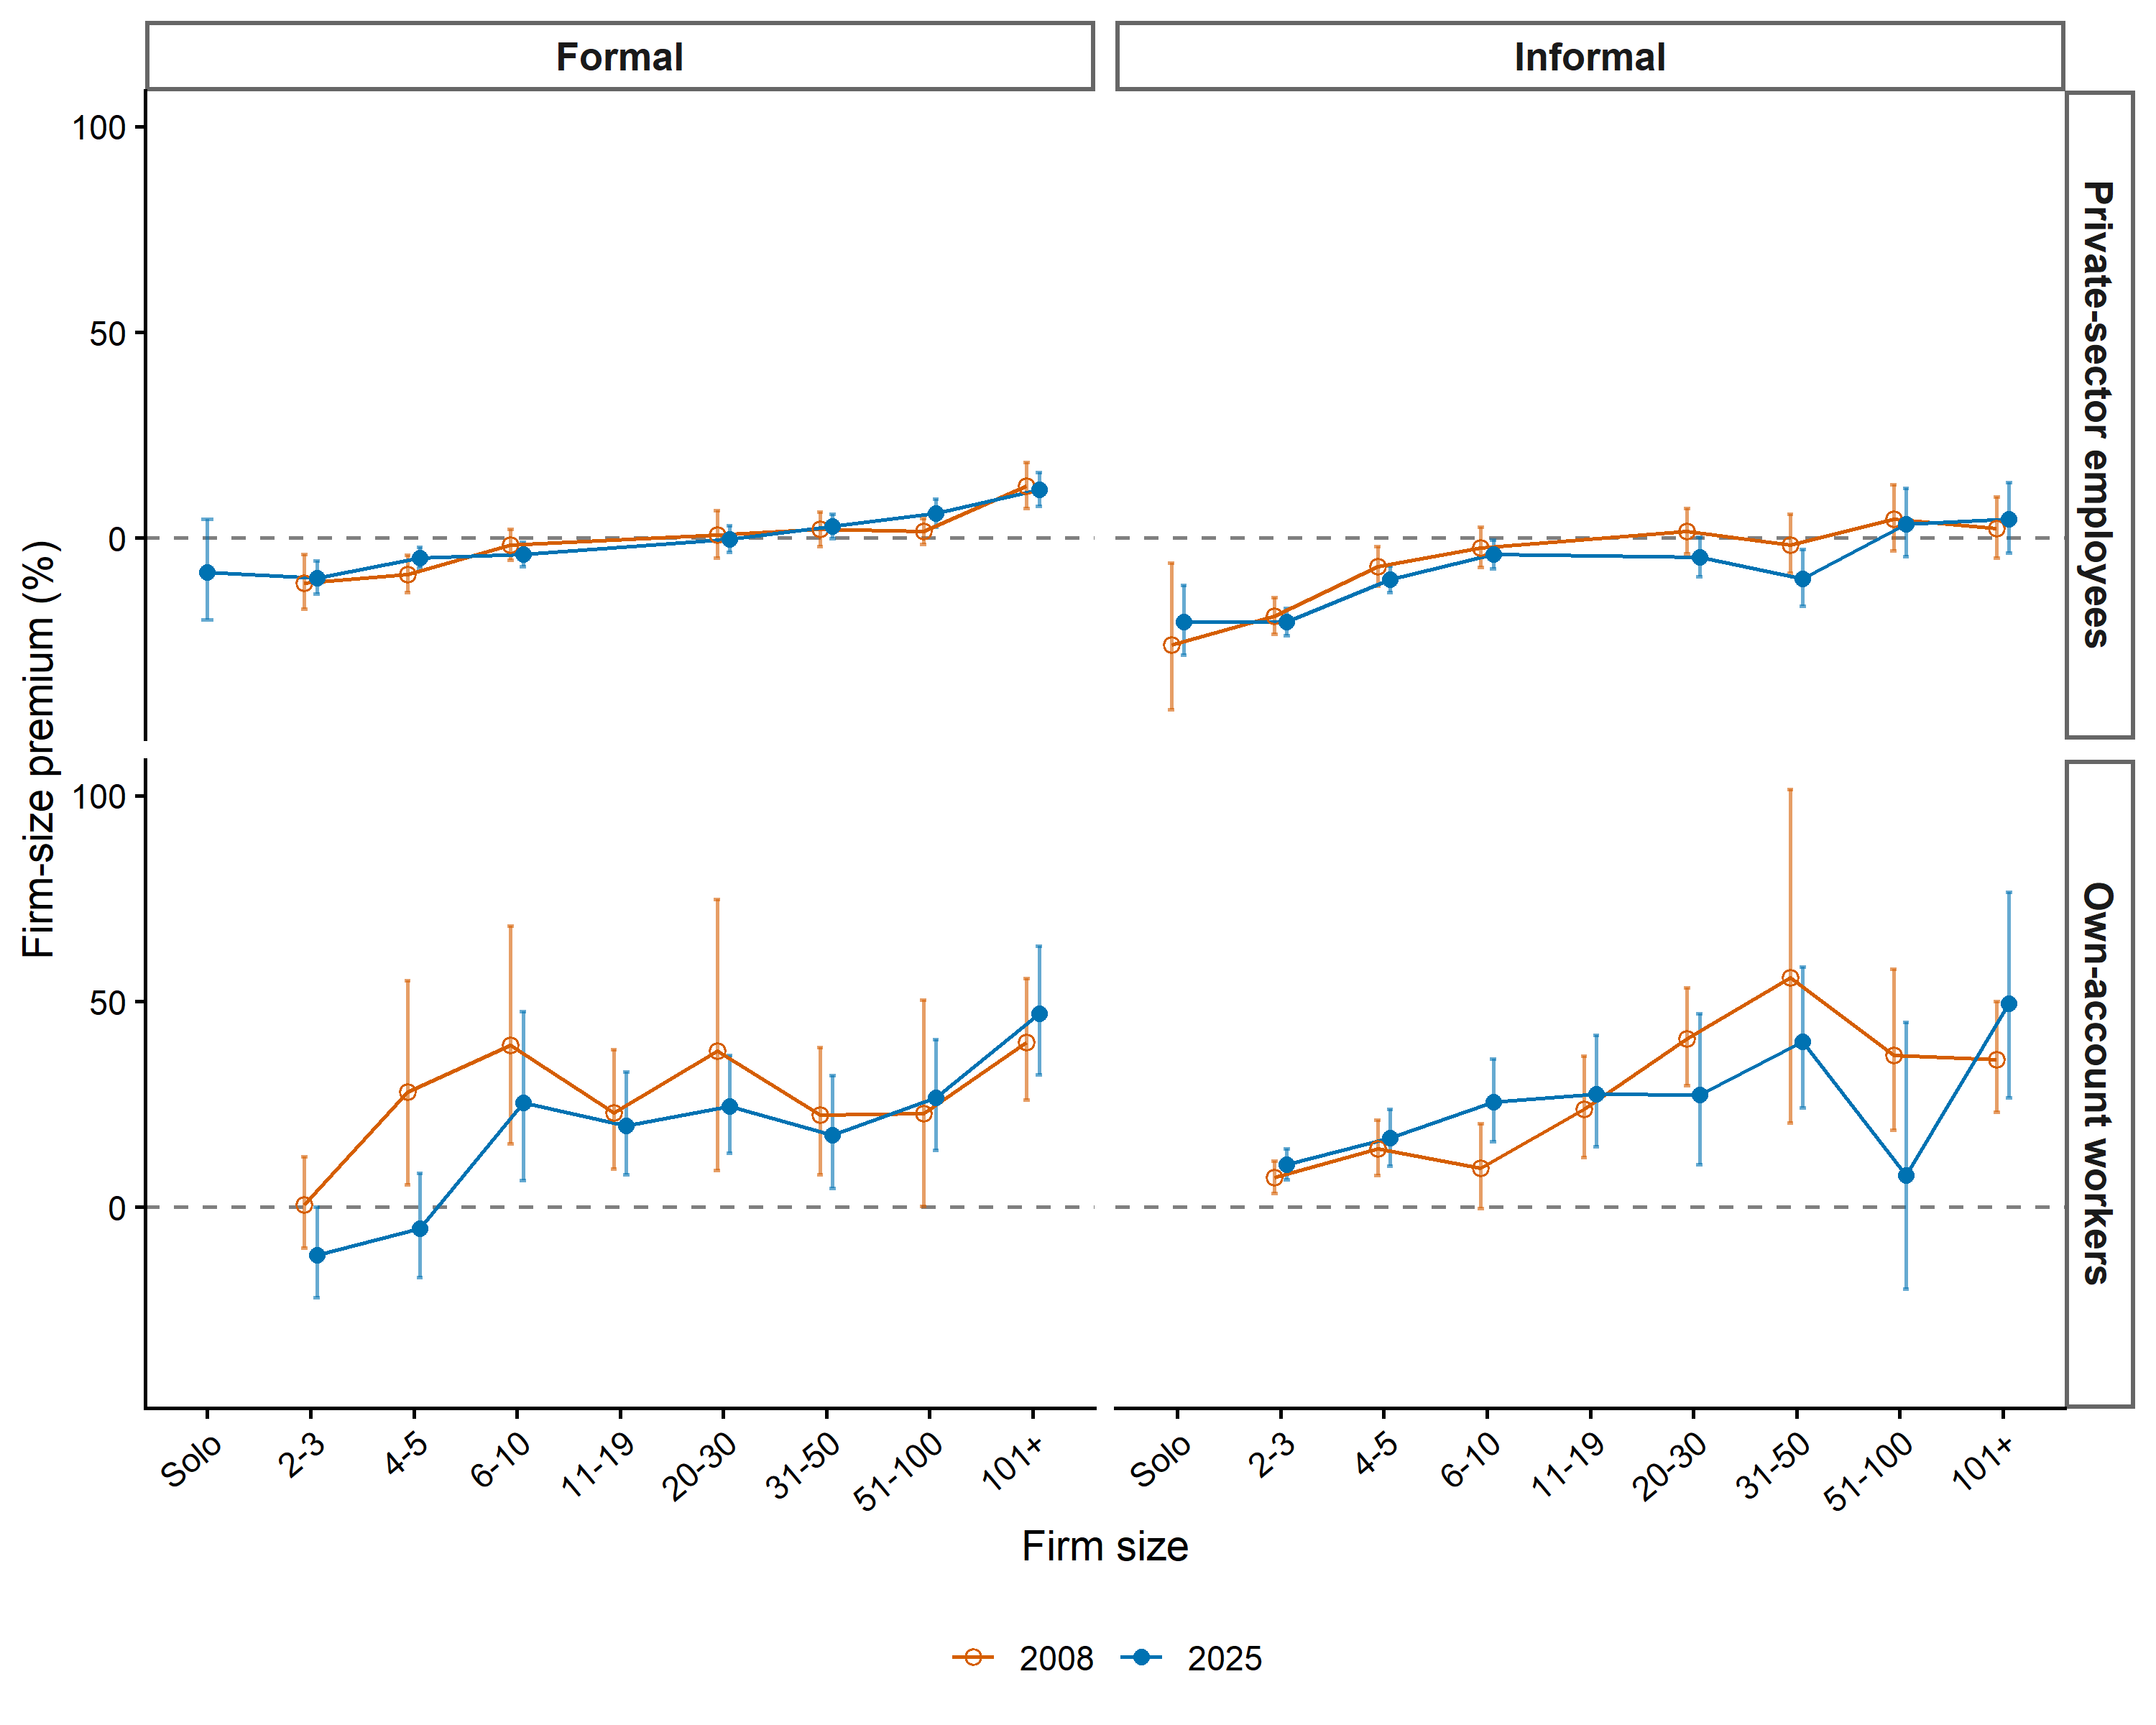
\includegraphics[width=\textwidth]{status_endpoints_en.png}
  \caption{M2 firm-size premiums by employment status and formality, 2008 and 2025}
  \label{fig:status-endpoints}
  \begin{minipage}{0.97\textwidth}\footnotesize
  Notes: The reference is 11--19 for private-sector employees and solo work
  for own-account workers, within formality and year. Points with fewer than
  30 observations at either endpoint are omitted. Bars are 95 percent confidence intervals using
  sector-department clustering.
  \end{minipage}
\end{figure}

Table~\ref{tab:status-endpoints} reports both reference categories and tests
changes using joint estimation of the two years. Relative to 11--19 workers,
the formal private-employee premium changes from 12.6 to 11.8 percent and
the informal premium from 2.3 to 4.6 percent. Relative to solo work, the
informal private-employee estimate falls from 38.2 to 31.3 percent. Among
own-account workers, the formal 101+/solo premium rises from 40.1 to
47.0 percent and the informal premium from 35.9 to 49.5 percent.
None of these changes is significant at 5 percent under sector-department
clustering. Using 11--19 as the reference for own-account workers also
produces insignificant endpoint changes.

\begin{table}[htbp]
\centering\small
\caption{M2 large-firm premiums under two references, 2008 and 2025}
\label{tab:status-endpoints}
\begin{tabular}{llrrrr}
\toprule
Status & Formality & 2008 (\%) & 2025 (\%) & Change (pp) & $p$-value \\
\midrule
\multicolumn{6}{l}{\textit{101+ relative to Solo}}\\
Private-sector employees & Formal & -- & -- & -- & -- \\
Private-sector employees & Informal & 38.2 & 31.3 & -6.9 & 0.711 \\
Own-account workers & Formal & 40.1 & 47.0 & 6.9 & 0.316 \\
Own-account workers & Informal & 35.9 & 49.5 & 13.6 & 0.311 \\
\midrule
\multicolumn{6}{l}{\textit{101+ relative to 11--19}}\\
Private-sector employees & Formal & 12.6 & 11.8 & -0.8 & 0.710 \\
Private-sector employees & Informal & 2.3 & 4.6 & 2.3 & 0.671 \\
Own-account workers & Formal & 14.0 & 22.8 & 8.8 & 0.295 \\
Own-account workers & Informal & 9.8 & 17.3 & 7.5 & 0.571 \\
\bottomrule
\end{tabular}
\par\vspace{0.3em}
\begin{minipage}{0.97\textwidth}\footnotesize
Notes: Equation~(\ref{eq:preferred-dynamics}). Changes in percentage points are computed before rounding. Two-sided tests compare endpoint log-wage contrasts using joint estimation and sector-department clustering. The formal private-employee solo comparison is omitted because its 2008 reference cell contains only eight observations.
\end{minipage}
\end{table}


Appendix Table~\ref{tab:status-endpoint-clustering} reports the tests under
sector, department, and two-way clustering, together with comparisons for
other employment categories. None of the reported private-employee or own-account
endpoint changes becomes significant at 5 percent under these alternatives.
Thus, the positive point estimate for informal own-account workers does not
establish a general widening of the informal premium. It coexists with a
negative point estimate among informal private-sector employees.

Figure~\ref{fig:status-dynamics} shows the annual paths from
Equation~(\ref{eq:preferred-dynamics}). The variation between adjacent years
also cautions against interpreting either endpoint difference as a steady
trend. The comparison retains employment categories, not the same workers,
so changes in unobserved composition within these categories can still matter.

\begin{figure}[htbp]
  \centering
  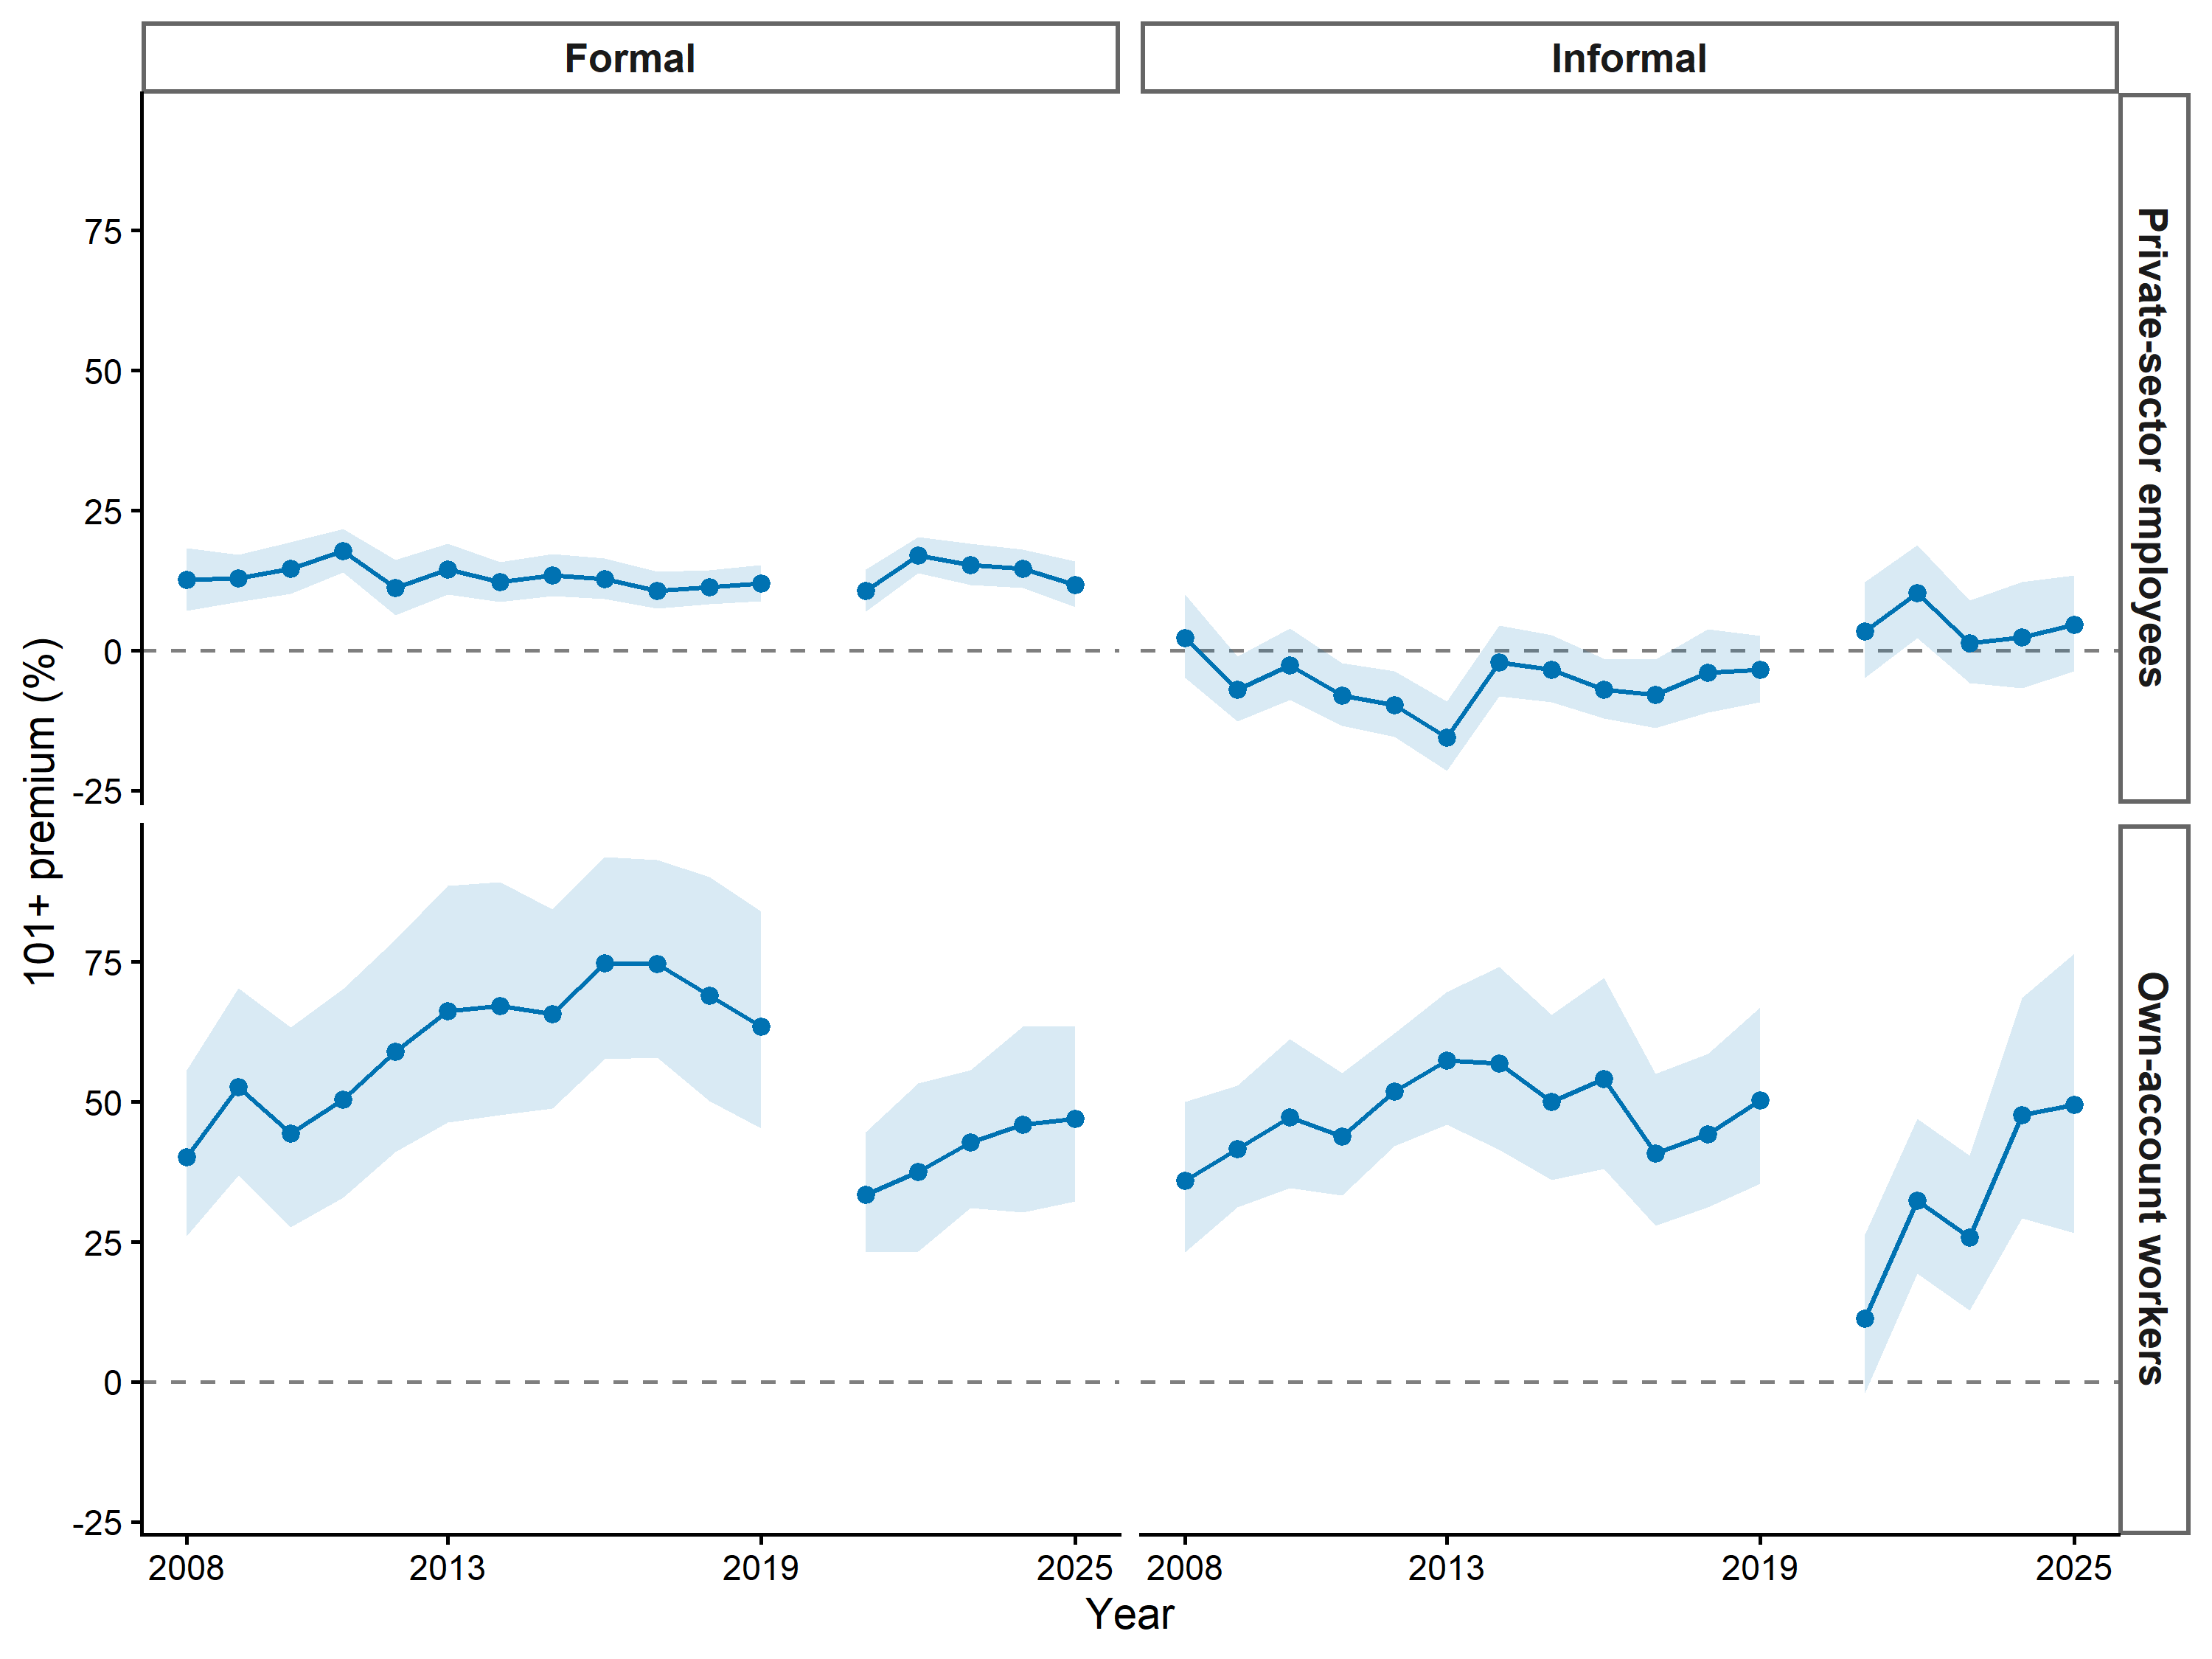
\includegraphics[width=\textwidth]{status_dynamics_en.png}
  \caption{Annual M2 large-firm premiums within employment and formality groups}
  \label{fig:status-dynamics}
  \begin{minipage}{0.97\textwidth}\footnotesize
  Notes: Premiums compare 101+ with 11--19 for private-sector employees and
  with solo work for own-account workers. Shaded areas are 95 percent
  confidence intervals using sector-department clustering. No estimate is
  reported for 2020.
  \end{minipage}
\end{figure}

\citet{BloomGuvenenSmithSongVonWachter2018} document a declining premium
in the United States, and \citet{reed2019large} find that it tends to
decline with national income and over time across developing economies.
Reed and Tran compare large firms with all firms below their threshold,
not only solo workers. \citet{ColonnelliTagWebbWolter2018} find no common
trajectory across Brazil, Germany, Sweden, and the United Kingdom.
Our M2 estimates do not establish either a common decline or a common
increase across employment and formality groups in Colombia.

The appendix retains simpler dynamic benchmarks for comparison.
Figure~\ref{fig:firm-size-wage-premium-over-time} reports the common-formality
model in Equation~(\ref{eq:dynamic-benchmark}).
Table~\ref{tab:firm-size-premium-trend-test} reports its linear-trend
version, Equation~(\ref{eq:trend-benchmark}), with alternative references
in Tables~\ref{tab:firm-size-premium-trend-test-101-reference} and
\ref{tab:firm-size-premium-trend-test-11-19-reference}.
Figures~\ref{fig:adjusted-formality-endpoints} and
\ref{fig:large-firm-formality-premium-over-time} show formality-specific
estimates with sector controls. Unlike M2, these models do not distinguish
size profiles by status in employment.
\FloatBarrier
